% ============================================================================
% Barycentre partiel
% Extrait de la fiche : Barycentres et lignes de niveau (classe de 1ere D)
% Necessite \usepackage{tikz} et \usetikzlibrary{calc} (charges par le fichier principal)
% ============================================================================
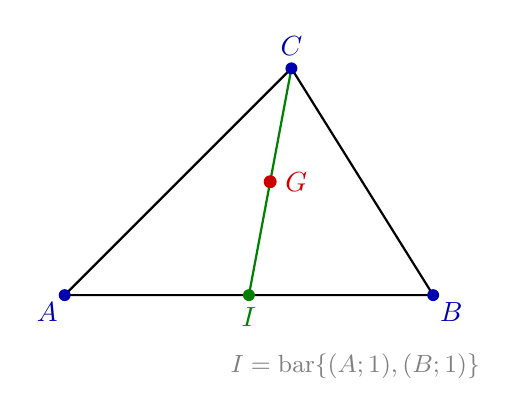
\begin{tikzpicture}[scale=0.9,>=latex]
  \coordinate (A) at (-2.6,0); \coordinate (B) at (2.6,0); \coordinate (C) at (0.6,3.2);
  \coordinate (I) at (0,0); \coordinate (G) at (0.3,1.6);
  \draw[thick] (A) -- (B) -- (C) -- cycle;
  \draw[thick,green!50!black] (I) -- (C);
  \fill[blue!70!black] (A) circle (2.4pt) node[below left=-1pt] {$A$};
  \fill[blue!70!black] (B) circle (2.4pt) node[below right=-1pt] {$B$};
  \fill[blue!70!black] (C) circle (2.4pt) node[above=1pt] {$C$};
  \fill[green!50!black] (I) circle (2.4pt) node[below=1pt] {$I$};
  \fill[red!80!black] (G) circle (2.6pt) node[right=2pt] {$G$};
  \node[font=\small,gray] at (1.5,-1.0) {$I=\mathrm{bar}\{(A;1),(B;1)\}$};
\end{tikzpicture}
